\documentclass[11pt]{beamer}
\usetheme{Madrid}
\usepackage[utf8]{inputenc}
\usepackage[french]{babel}
\usepackage[T1]{fontenc}
\usepackage{amsmath}
\usepackage{amsfonts}
\usepackage{amssymb}
\usepackage{graphicx}
\usepackage{tikz}
\author{Matthieu Brachet}
\title{Climatologie et Imagerie 3D}

\begin{document}

\begin{frame}
\titlepage
\includegraphics[scale=0.3]{iecl.jpg}
\end{frame}

\begin{frame}
\tableofcontents
\end{frame}

\begin{frame}
\begin{center}
Climatologie.
\end{center}
\end{frame}

\section{Applications au climat}
\subsection{Contexte}
\begin{frame}{Contexte}
\begin{columns}
\column{0.45\textwidth}
\begin{block}{Actualité}
\begin{itemize}
\item Réchauffement climatique,
\item GIEC,
\item COP22,
\item ...
\end{itemize}
\end{block}

\column{0.45\textwidth}
\begin{center}
\includegraphics[scale=0.2]{earth.png}
\end{center}
\end{columns}

\begin{block}{Problème général}
Comment prévoir le climat de la Terre?
\end{block}
\end{frame}

\subsection{Problème général}
\begin{frame}
\begin{block}{Problèmatique}
Prédiction du climat d'une planète

\begin{flushright}
$\Rightarrow$ Modèlisation mathématique : écriture en language mathématique d'un problème issu de la physique.
\end{flushright}

\pause
\end{block}

\vspace{0.8cm}
\begin{columns}
\column{0.45\textwidth}
Paramètres du problème :
\begin{itemize}
\item Equations de changement d'état,
\item Effet de serre,
\item Circulation atmosphèrique,
\item Circulation océanique,
\item ...
\end{itemize}

\pause
\column{0.45\textwidth}
\begin{block}{}
Ecriture d'un modèle de circulation générale.
\end{block}
\end{columns}
\end{frame}

\begin{frame}
\textbf{Morceau du modèle de circulation générale :} eq. Shallow Water
\begin{equation}
\left\lbrace
\begin{array}{rcl}
\dfrac{\partial h^{\star}}{\partial t} + \nabla \cdot \left( h^{\star} \mathbf{u} \right) & = & 0 \\
\dfrac{\partial \mathbf{u}}{\partial t} + \nabla \left( \dfrac{1}{2} \mathbf{u}^2 + g h \right) + \left(f  + \left( \nabla \wedge \mathbf{u} \right) \cdot \mathbf{k}\right) \mathbf{k} \wedge \mathbf{u} & = & \mathbf{0}
\end{array}
\right.
\end{equation}

\pause
\textbf{Prévisions :}

\begin{center}
\includegraphics[scale=0.3]{gwprediction.png}
\end{center}
\end{frame}

\begin{frame}
\begin{center}
Comment?
\end{center}
\end{frame}


\subsection{Méthode}
\begin{frame}{Méthode}
\begin{block}{}
Résolution par ordinateur
\end{block}
\pause

\begin{block}{Ordinateur :}
\begin{itemize}
\item mémoire finie : nombre fini de décimales,
\item pas de temps continu,
\item besoin de discrétiser.
\end{itemize}
\end{block}
\pause

\begin{block}{But :}
Méthode \textbf{rapide} et \textbf{précise}.
\end{block}
\end{frame}

\begin{frame}

\begin{block}{Idée :}
\textbf{Calcul d'une vitesse :}
\begin{equation}
v = \dfrac{D}{T}
\end{equation}
\end{block}

\pause
$$\dfrac{S(\text{maintenant}) - S(\text{juste avant})}{\text{durée}} = \text{évolution}$$

\pause
\begin{center}
\begin{tikzpicture}[scale=1]
\draw [>=latex,->] (0,0) -- (8,0);
\draw (0,0) node[below] {0 sec} node{$\bullet$};
\draw (1.5,0) node[below] {5 sec} node{$\bullet$};
\draw (3,0) node[below] {10 sec} node{$\bullet$};
\draw (6,0) node[below] {1 h} node{$\bullet$};
\draw [>=latex,->] (1.5,0.2) arc (180:0:0.75) ;
\end{tikzpicture}
\end{center}

C'est la \textbf{discrétisation} (ici discrétisation en temps).

\end{frame}

\begin{frame}{Pour l'atmosphère :}

\begin{block}{Discrétisation}
\begin{itemize}
\item discrétisation en temps,
\item grillage sur la sphère.
\end{itemize}
\end{block}

\begin{figure}
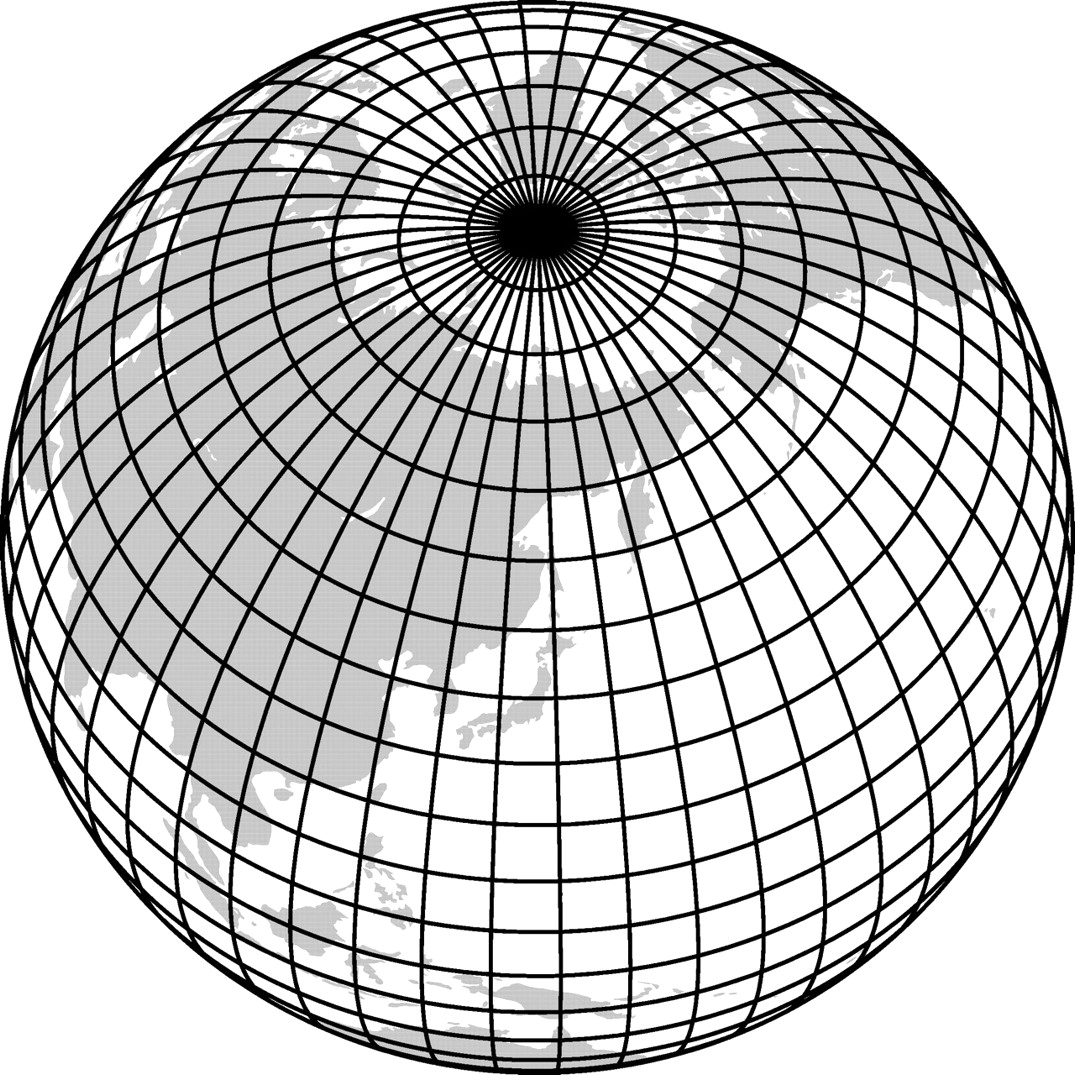
\includegraphics[height=3cm]{lonlat_grid.jpg} \hspace{1cm}
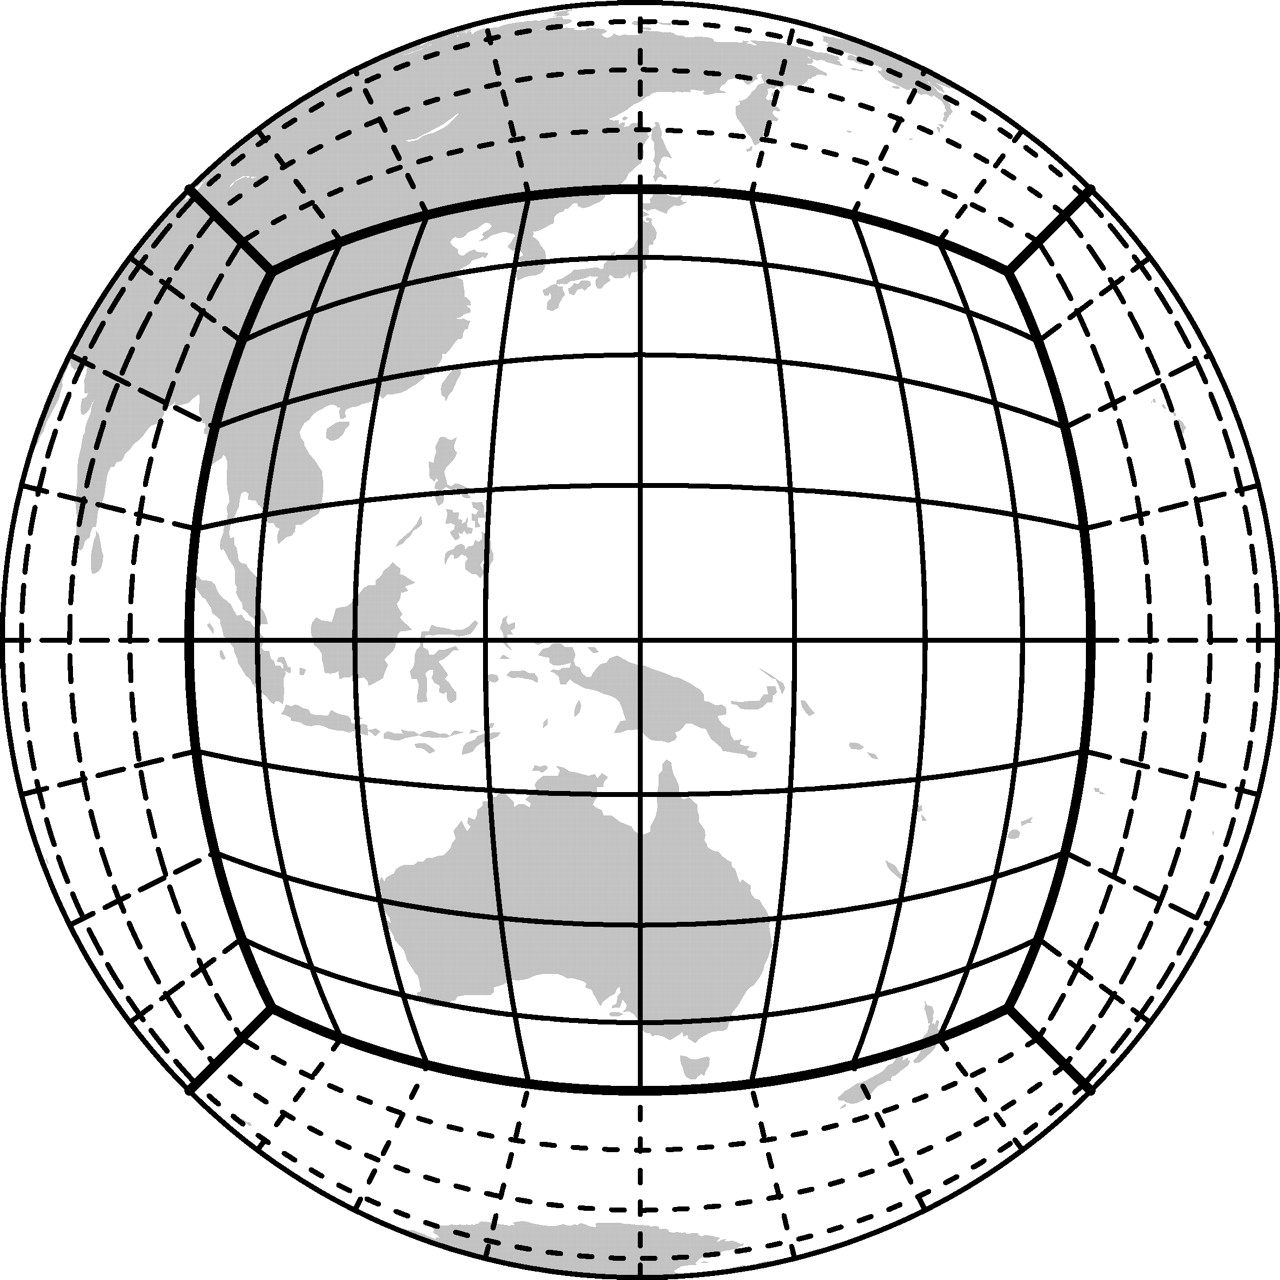
\includegraphics[height=3cm]{CS_grid.jpg}
\caption{Quelques maillages de la sphère}
\end{figure}

\end{frame}

\begin{frame}{Bilan :}
\begin{columns}
\column{0.45\textwidth}
\begin{block}{}
\begin{itemize}
\item Calcul de la solution aux "noeuds" du grillage,
\item Calcul à des temps fixés (nombreux).
\end{itemize}
\end{block}

\column{0.45\textwidth}
\begin{center}
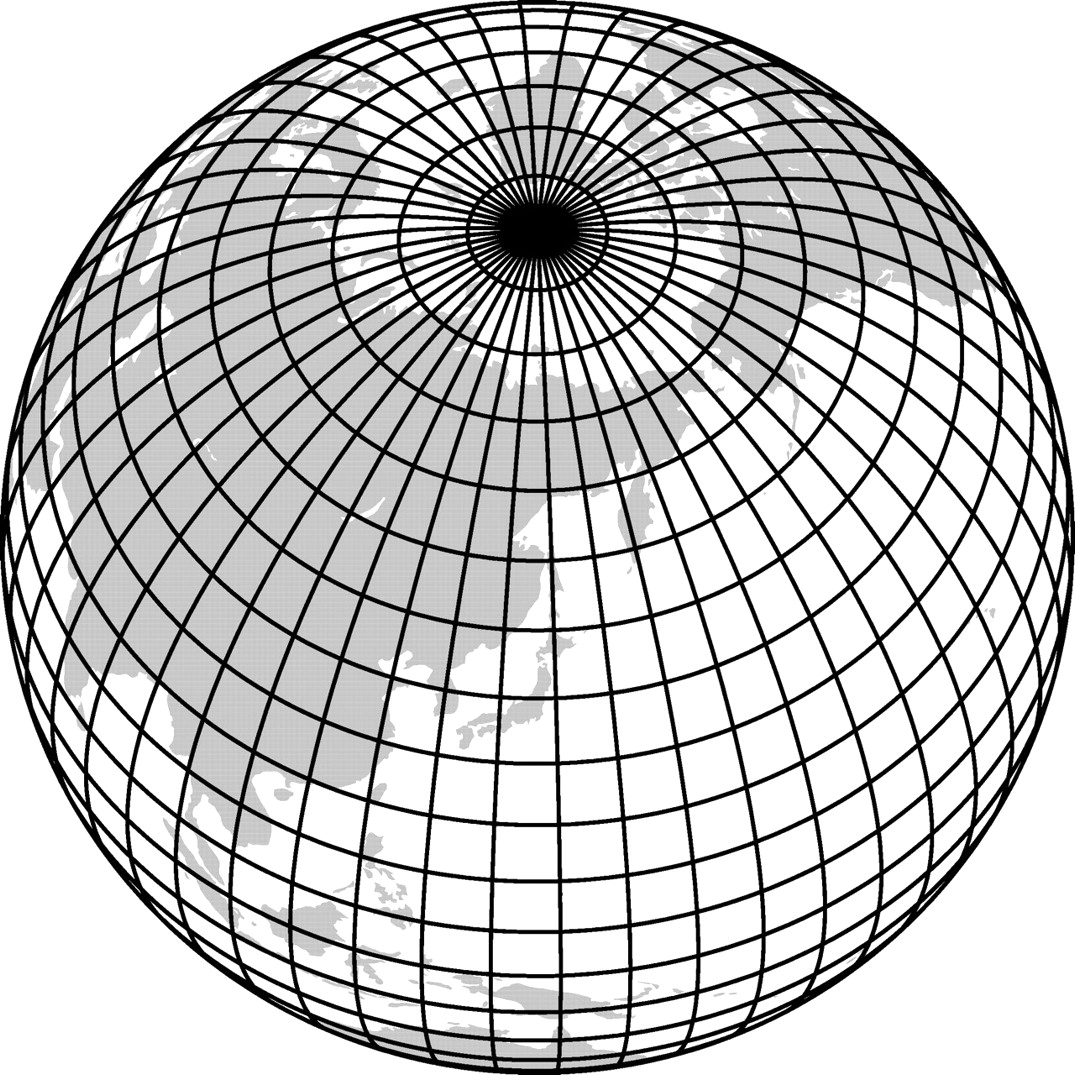
\includegraphics[height=3cm]{lonlat_grid.jpg} 
\end{center}
\end{columns}
\end{frame}

\begin{frame}

\begin{block}{Travail}
Augmentation progressive de la difficulté des tests.
\end{block}

\pause

\begin{block}{Questions mathématiques :}
\begin{itemize}
\item Quelle précision?
\item Stabilité ?
\item Conservation de la matière? de l'énergie?
\end{itemize}
\end{block}

\begin{center}
\href{run:ref_7363145849_test_2.avi}{\includegraphics[scale=0.2]{14-Oct-2015_normerreur_test_2.png}} 
\href{run:ref_7366568562.avi}{\includegraphics[scale=0.18]{relief.jpg}}
\end{center}

\end{frame}


\begin{frame}
\begin{center}
Imagerie.
\end{center}
\end{frame}


\section{Applications en imagerie 3D}
\subsection{Contexte}
\begin{frame}{Contexte}
\textbf{Projet E-Cathédrale :}
\begin{columns}
\column{0.45\textwidth}
\begin{block}{}
Construction d'un modèle 3D de la cathédrale d'Amiens
\end{block}
\begin{alertblock}{}
Données manquantes...
\end{alertblock}
\column{0.45\textwidth}
\begin{center}
\includegraphics[scale=0.2]{cathedrale-amiens-3.jpg}
\end{center}
\begin{tiny}
\begin{flushright}
\textit{Source : Projet E-cathédrale}
\end{flushright}
\end{tiny}
\end{columns}
\end{frame}


\begin{frame}
\textbf{GPS :}
\begin{columns}
\column{0.45\textwidth}
\begin{block}{}
Utilisations de données satellites pour la cartographie.
\end{block}
\begin{alertblock}{}
Données manquantes...
\end{alertblock}
\column{0.45\textwidth}
\begin{center}
\includegraphics[scale=0.2]{sat1.jpg}
\end{center}
\end{columns}
\end{frame}

\subsection{Problème général}
\begin{frame}{Constitution d'une image}
A chaque pixel on associe un nombre

\begin{center}
\includegraphics[scale=0.15]{lion.jpg}
\includegraphics[scale=0.16]{imbin.jpg}
\end{center}

Pour une image binaire : que des 1 et des -1 (objet ou pas objet).

\end{frame}

\subsection{Méthode}
\begin{frame}{Modèle de reconstruction}
Utilisation d'un modèle mathématique qui :

\begin{itemize}
\item Conserve les données fiables de l'image,
\item Reconstruit de manière logique les données manquantes.
\end{itemize}
\pause
\vspace{0.8cm}
Utilisation d'équations issues de la biologie (développement de tumeurs) dont les propriétés mathématiques sont intéressantes.

\pause
\vspace{0.8cm}
\begin{center}
\fbox{Image initiale} $\Rightarrow$ \fbox{Image un peu corrigée} $\Rightarrow$ \fbox{un peu plus ...} $\Rightarrow$ ...
\end{center}
\end{frame}

\begin{frame}
\begin{center}
Application en 2D
\end{center}
\end{frame}

\begin{frame}
\begin{center}
\href{run:ref7365716039_date29-Aug-2016_test4.avi}{\includegraphics[scale=0.25]{carre.png}}
\end{center}
\end{frame}

\begin{frame}
\begin{center}
Application en 3D
\end{center}
\end{frame}


\begin{frame}
\begin{center}
\includegraphics[scale=0.3]{im3d0.jpg}
\end{center}
\end{frame}

\begin{frame}
\begin{center}
\includegraphics[scale=0.3]{im3d1.jpg}
\end{center}
\end{frame}

\begin{frame}
\begin{center}
\includegraphics[scale=0.3]{im3d2.jpg}
\end{center}
\end{frame}

\begin{frame}
\begin{center}
\includegraphics[scale=0.3]{im3d4.jpg}
\end{center}
\end{frame}

\begin{frame}
\begin{center}
\includegraphics[scale=0.3]{im3d5.jpg}
\end{center}
\end{frame}

\section{Bilan}
\begin{frame}{Bilan}
Méthode utilisée ici :
\begin{enumerate}
\item Apprentissage du problème,
\item Modélisation mathématique,
\item Resolution.
\end{enumerate}

Applications de l'analyse numérique en imagerie 2D et 3D et en climatologie.

\end{frame}

\begin{frame}
\begin{center}
Merci de votre attention :)
\end{center}
\end{frame}


\end{document}
